\documentclass{article}
\usepackage[letterpaper]{geometry}
\geometry{verbose,tmargin=1in,bmargin=1in,lmargin=1in,rmargin=1in}

\usepackage[utf8]{inputenc}
\usepackage{amsmath}
\usepackage{float}
\usepackage{listings}
\usepackage{graphicx}
\usepackage{enumitem}
\usepackage[bbgreekl]{mathbbol}

\renewcommand{\baselinestretch}{1.5}

\title{CIS 419/519: Homework 6}
\author{\{Yupeng Li\}}
\date{04.15.2020}

\begin{document}
    \maketitle
    Although the solutions are entirely my own, I consulted with the following people and sources while working on this homework: \textbf{https://www.youtube.com/watch?v=kNPGXgzxoHw}
    \paragraph{PART I: PROBELM SET}
    \section{Reinforcement Learning I}
    The reward does not communicate the goal to the robot well. The robot can only get a positive reward at the end of the maze while all the other points have 0 reward. That is to say, the robot does not know what to do until it first reaches the exit and it keeps wandering around before that. A better reward would be giving all the failed runs a negative reward so that the robot would know that it should try to navigate to the exit as quick as possible.
    \section{Reinforcement Learning II}
\textbf{(a)} The signs do not matter in continuing tasks. For episodic tasks, however, the sign of these rewards do matter as in problem I.\\\\
\textbf{(b)} Based on the fact that:
\[R_{t} = \sum_{k=0}^{\infty} \gamma^{k} r_{t+k+1}\]
Adding a constant C to all the rewards will simply yield a new reward $\tilde{R_{t}}$ such that:
\[\tilde{R_{t}} = \sum_{k=0}^{\infty} \gamma^{k} (r_{t+k+1} + C)\]
which is also equivalent to:
\[\sum_{k=0}^{\infty} \gamma^{k} (r_{t+k+1}) + \sum_{k=0}^{\infty} C \gamma^k\]
That is to say:
\[\tilde{R_{t}} = R_{t} + \sum_{k=0}^{\infty} C \gamma^k \]
Putting this in to the Value function $V^{\pi}(s) = \mathbb{E}_{\pi} [R_{t}\mid s_t =s]$\\
We can easily obtain the fact that 
\[\tilde{V}_{\pi}(s) = \mathbb{E}_{\pi} [G_{t} + \sum_{k=0}^{\infty} \gamma^k C \mid S_t = s] = V_{\pi} (s) + \sum_{k=0}^{\infty} \gamma^k C\]
Since the discounted factor $\gamma$ is always smaller than 1, the second term in the equation above can be simplified as $\frac{C}{1-\gamma}$ based on the geometric series sum.\\\\
\textbf{(c)} Based on the facts above, that is to say, the constant K added to the values of all states is simply 
\[\frac{C}{1-\gamma}\]
\paragraph{PART II: PROGRAMMING EXERCISES}
\section{Random policy for the MountainCar gym environment}
\textbf{(i)} The action spaces consist of three discrete actions each regarding to accelerate to left, accelerate to right and stay still. The observation space is a two dimensional space each of which represents x or y coordinate of the mountain car.\\\\
\textbf{(ii)} The mean reward obtained over 10 episodes remain to be -200 since the car never got to the goal based on a random policy within 200 steps.

\section{Train a Q-learner and generate expert trajectories}
The function \textbf{discretize()} turns the infinite set of combinations of the observation space into discretized finite states and round the infinite state to its closest. Increasing the discretization argument  will increase the model size since there would be more possible observation states.
\section{Train an imitation policy}

The loss and success rate of 20 episodes with 2 epochs are in the following figure
		\begin{figure}[H]
			\caption{20 Episodes and 2 Epochs}
			\centering
			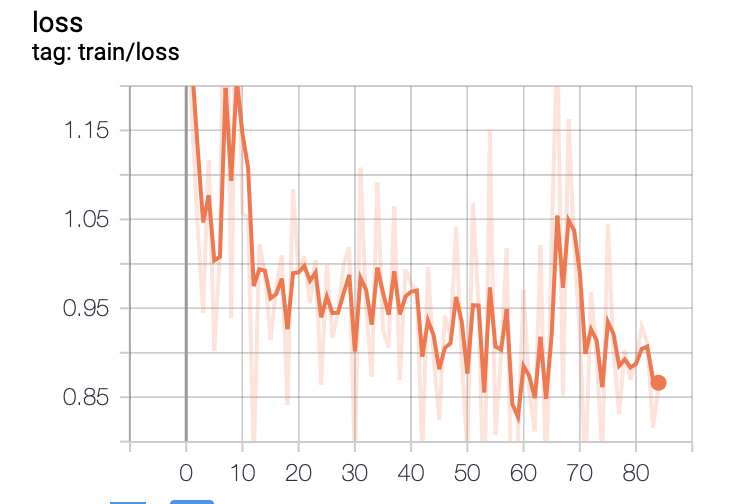
\includegraphics[width=8cm]{lossinit20ep2.png}
		\end{figure}
Since there are only 2 epochs, the data is too little to plot out for success rate reward
The loss and success rate of 2 episodes with 20 epochs are in the following figure
		\begin{figure}[H]
			\caption{2 Episodes and 20 Epochs loss}
			\centering
			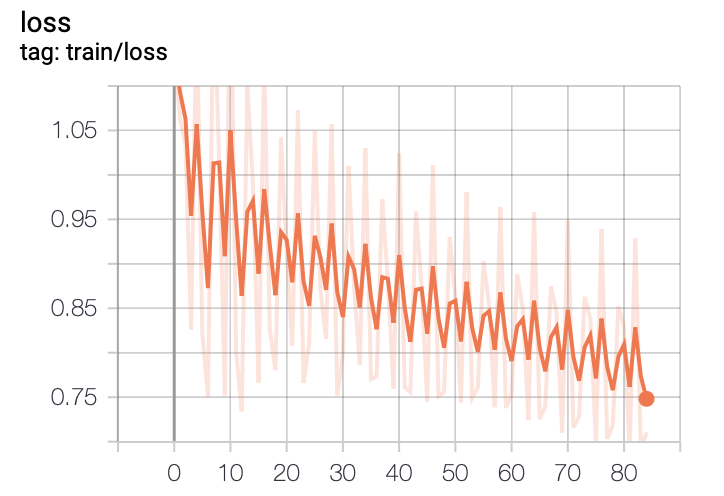
\includegraphics[width=8cm]{vanillainit2ep20.png}
		\end{figure}
The average reward and average success follows:
		\begin{figure}[H]
			\caption{2 Episodes and 20 Epochs Reward and Success}
			\centering
			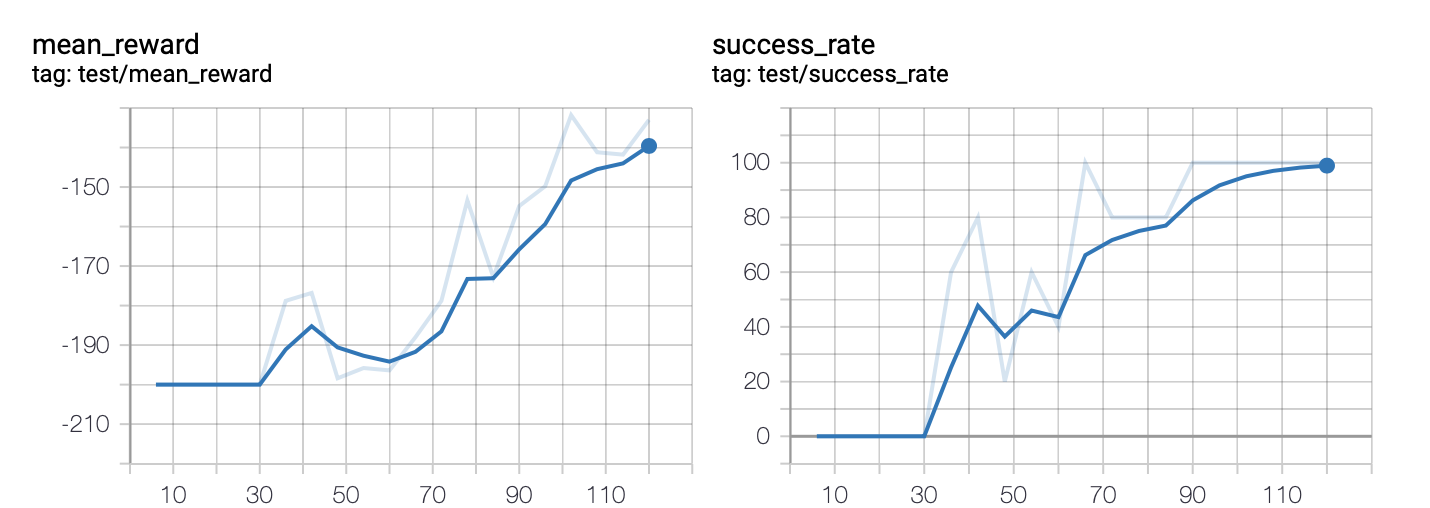
\includegraphics[width=8cm]{rewardinit2ep20.png}
		\end{figure}
\section{Implement DAgger}
After implementing DAgger, the performance of the model further improves as in the following picture:
		\begin{figure}[H]
			\caption{DAgger loss, reward and success}
			\centering
			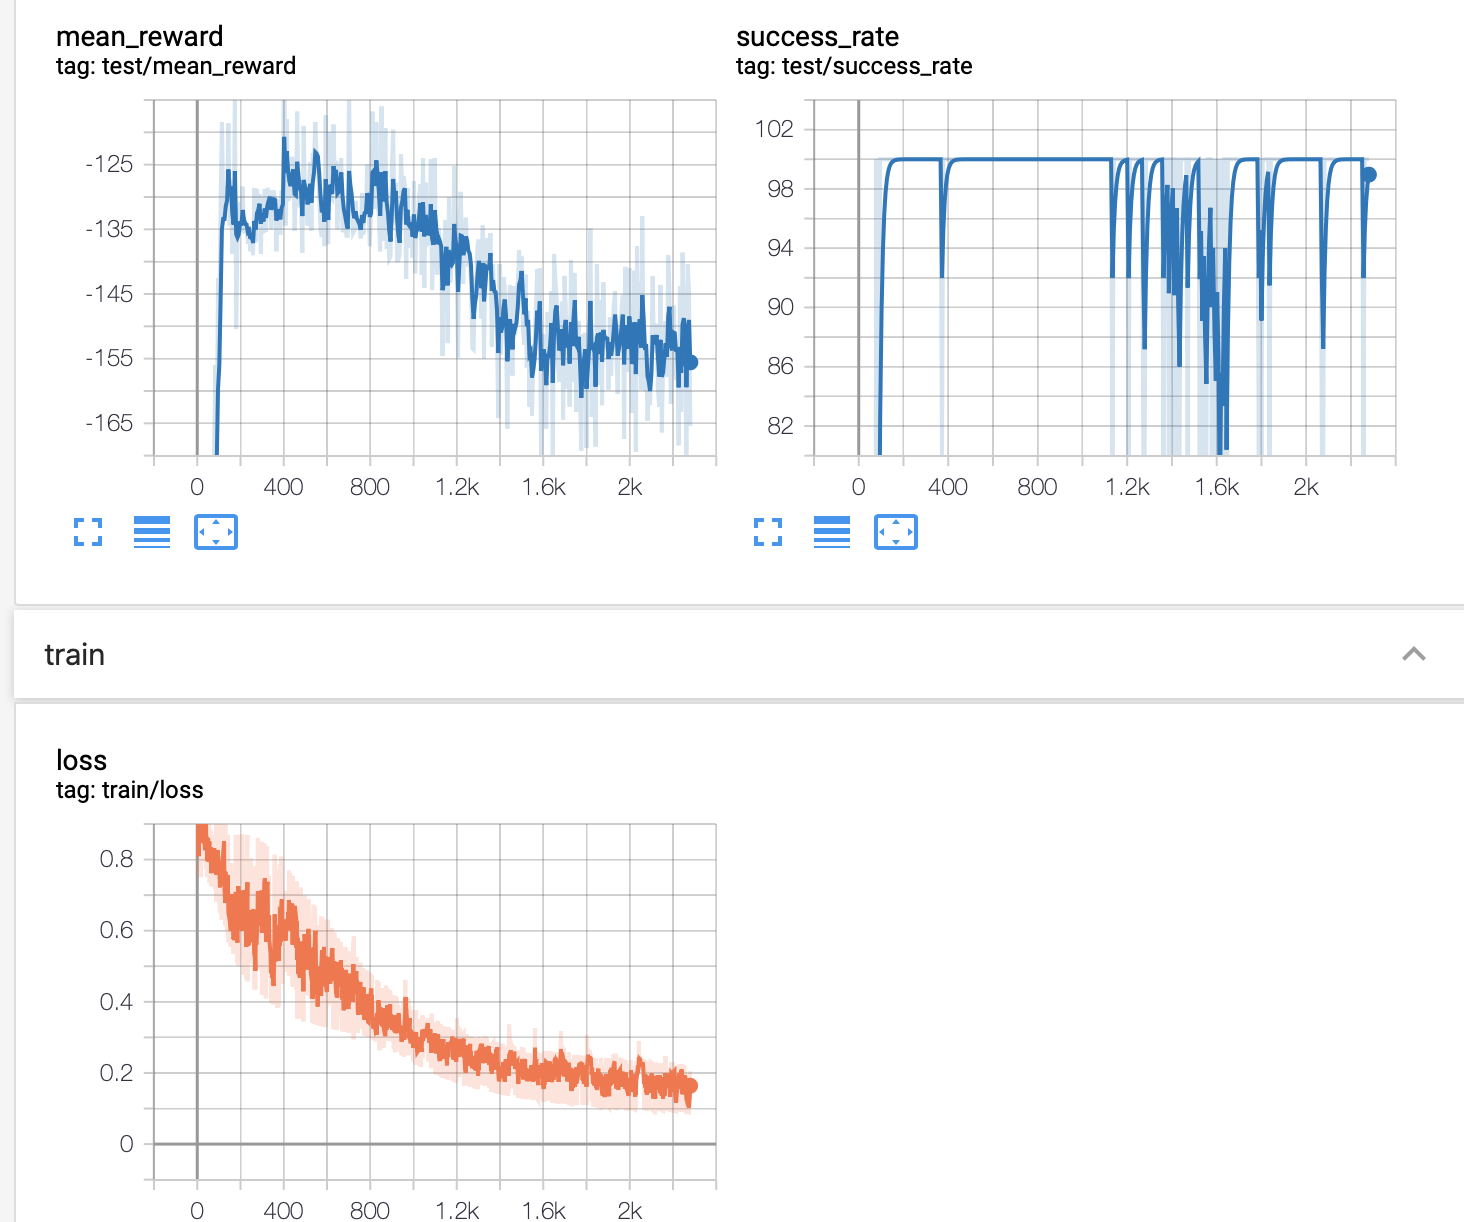
\includegraphics[width=8cm]{Dagger.png}
		\end{figure}
\end{document}